\chapter{Implementation and experiments}\label{cha:results}

\section{Implementation details}
The following sections describe relevant details regarding the implementation of the proposed method.

\subsection{Obstacle avoidance}
To ensure low execution times it is crucial to use an efficient method of checking for collisions between states and $\xobst$. 
In this implementation, the S2Geometry library developed by Google was used \cite{s2geo}. This is a C++ library which contains 
efficient methods to index geometrical objects of any shape, and checking for collisions between different geometries such as points, lines and polygons. 

\subsection{Input set generation}
The input set $\inputs$ was generated using the approach described in Section \ref{sec:motion_prims_wind}. 
It was generated for wind directions $\psi_{w,s}=\{0\degree,20\degree,40\degree,\hdots,340\degree\}$ and desired final course changes
$\Delta\cog=\{20\degree,40\degree,\hdots,180\degree\}$, resulting in a total of 162 inputs for each specific $\windspd$. Symmetries of the system reduce the set of necessary inputs
as solutions for $\Delta\cog=\{-20\degree,-40\degree,\hdots,-180\degree\}$ are simply found by mirroring the $y_E$ coordinate of $u$.
The optimization problem was solved using \textabbr{nomad} \cite{nomad}, a C++ implementation of the \ac{mads} algorithm introduced in Section \ref{sec:solve_opt_ctrl}.
Cross-track error constraints were defined by $\lambda_d=25$ and $d_{\text{min}}=2.5$ m, \ac{cog} error $\Delta\psi=15\degree$ and wind variation $\delta_W=0.25$. The initial guess for $u$ 
was found by performing a grid search over the values
\begin{equation}
    \actions_{s,\text{init}}=\{(\Delta x_N,\Delta y_E): |\Delta x_N| \leq 300, 0\leq \Delta y_N \leq 300\}
\end{equation}
with a step size of 10 meters and selecting the input with the lowest value of the objective in Equation \eqref{eq:max_opt}.
Simulations of the closed-loop system for the generated inputs $u$, calculated for some different wind directions and $\windspd\in[3.75, 6.25]$ m/s, are shown in Figure \ref{fig:motion_prims}.
\begin{figure}
    \centering
    \subfloat[Inputs generated for $\winddir=0\degree$]{
        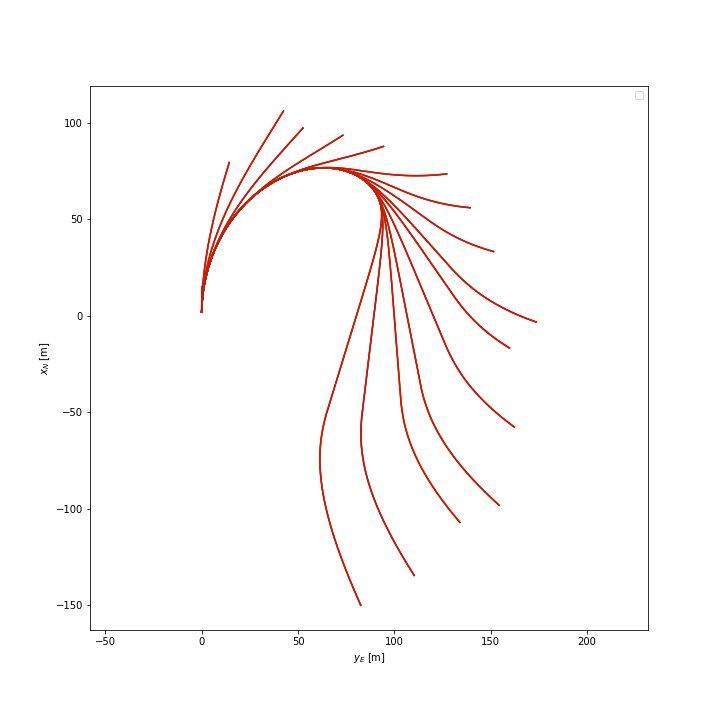
\includegraphics[width=.8\linewidth]{mp_0}
    }\\
    \subfloat[Inputs generated for $\winddir=80\degree$]{
        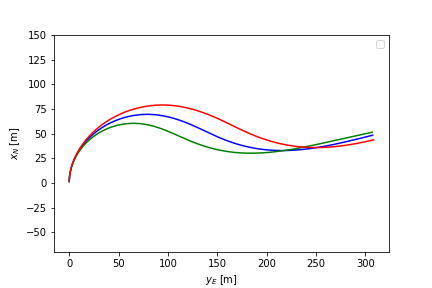
\includegraphics[width=.8\linewidth]{mp_80}
    }
    \caption{Inputs for different wind directions, $\windspd\in[3.75, 6.25]$ m/s}
    \label{fig:motion_prims}
\end{figure}

\subsection{State-space discretization}
To apply graph-search methods, the state-space has to be discretized. In this work the values of $x_N$ and $y_E$ were discretized into cells of size $d=10$ meters, and the 
heading $\psi$ was discretized in steps of $20\degree$. The Hybrid $A^*$ method presented in Section \ref{sec:hybrid-a-star} was used when sampling the state space, allowing continuous values of the state vector $x$ but assigning those to the closest 
discretized state.

\subsection{State expansions}
The step $\text{EXPAND}$ in Algorithm \ref{alg:astar} presented in Section \ref{sec:a-star} has to take both the wind direction $\winddir$ and the heading $\psi$ of $x$ into account. 
Since the inputs in $\inputs$ are generated using initial course $\cog=0$, it is first necessary to calculate the closest relative wind direction
\begin{equation}
    \psi_{w,\text{rel}}=\argmin_{\psi_{w,s}\in\{\psi_{w,s}\}}|(\psi-\winddir)-\psi_{w,s}|
\end{equation}
which is used to select the inputs for expansion. When mirroring inputs the wind direction also has to be mirrored, \ie\ 
$\tilde{\psi}_w=360\degree-\winddir$ is used to calculate $\psi_{w,\text{rel}}$. The selected inputs also have to be rotated, \ie\ the initial reference $u=(\Delta x_N, \Delta y_E)$ is transformed to 
\begin{equation}
    \tilde{u}=(\cos\psi \Delta x_N + \sin\psi \Delta y_E, -\sin\psi \Delta x_N + \cos\psi \Delta y_E)
\end{equation}
Finally, the expanded states and corresponding costs are found by simulating the closed-loop system \eqref{eq:closed_loop} using each selected $\tilde{u}$ as input. 
The actual wind direction $\winddir$ is used instead of $\psi_{w,s}$ in these simulations.

\subsubsection{Handling perpendicular winds}
A drawback of using straight line-segments as the control reference is that some inputs become problematic when the difference between 
$\psi$ and $\winddir$ is close to $90 \degree$. In this situation, expanding using an input which corresponds to a course change 
 of $\Delta\cog\approx180\degree$ might result in the trajectory controller choosing to fly in tailwind instead of headwind, leading to a large cross track error. This situation is 
 illustrated in Figure \ref{fig:hdg_diff_wind}.

\begin{figure}
    \begin{center}
        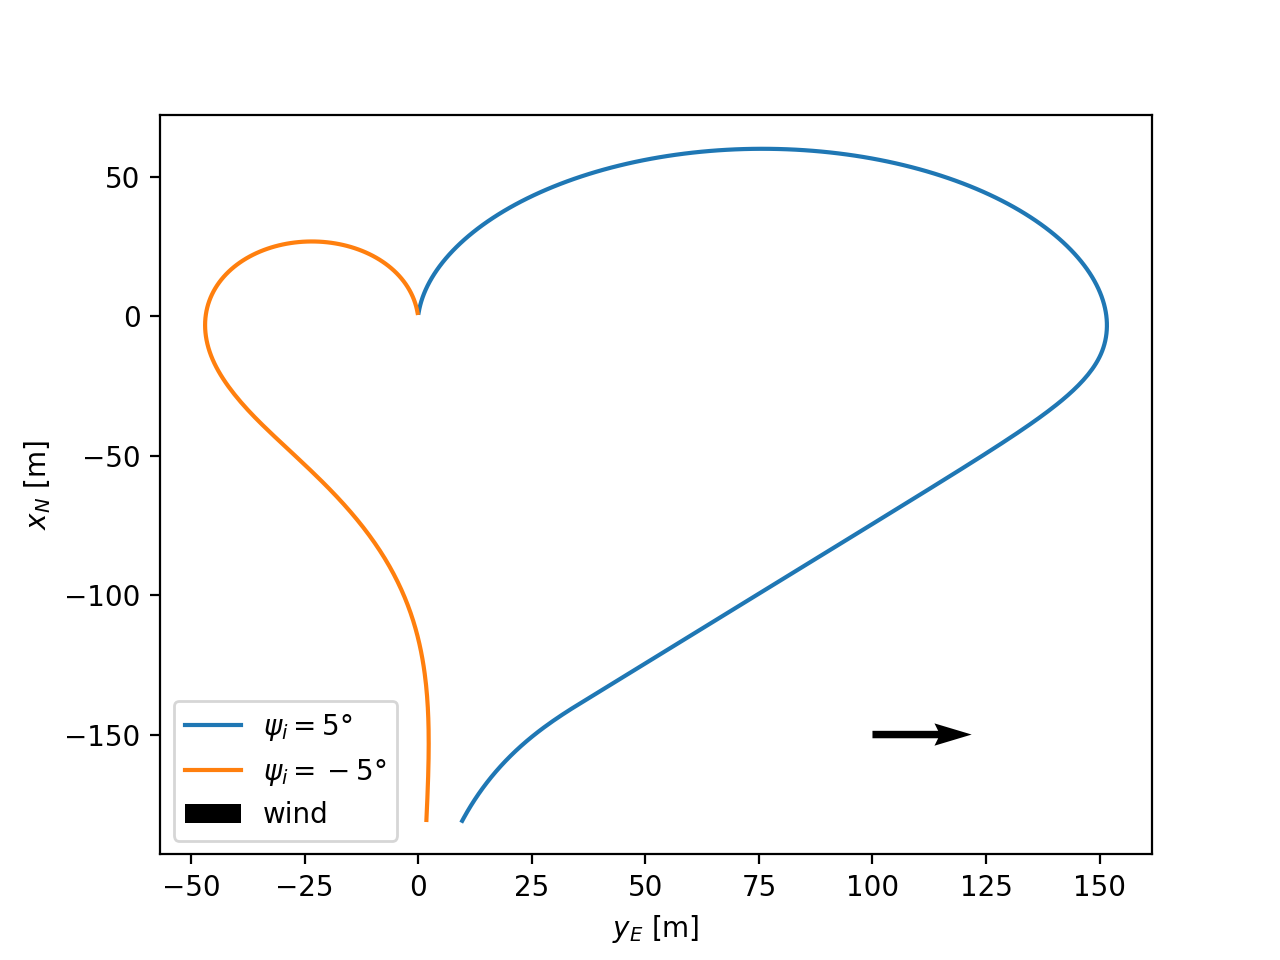
\includegraphics[width=.7\linewidth]{fig/prim_diff_hdg}        
    \end{center}
    \caption{Large cross track error for $\Delta\cog\approx180\degree$ when the wind is perpendicular to \ac{uav} motion}
    \label{fig:hdg_diff_wind}
\end{figure}

This issue was mitigated by defining a set $\psi_{\text{safe}}$ as 
\begin{equation}
    \psi_{\text{safe}}=\{\psi: |\sin\psi|<\frac{1}{\sqrt{2}}\}
\end{equation}
If $|\psi-\winddir|\notin\psi_{\text{safe}}$ during expansion only inputs corresponding to $|\Delta\cog|\leq160\degree$ are used.

\subsection{Heuristic Lookup Table}
The \ac{hlut} was generated using the method in Algorithm \ref{alg:hlut} presented in section \ref{sec:hlut}, using the wind-direction $\winddir=0$. This implies that 
entries have to be generated for initial values of $\psi$ from $0\degree$ to $180\degree$ to cover all possible situations. To query a stored heuristic value $\tilde{h}(x, \tilde{x})$ it is 
thus necessary to rotate both $x$ and $\tilde{x}$ by the angle $\winddir$ in order for the query to align with the \ac{hlut}. 

The set of states for which to generate entries was selected as 
\begin{equation}
    \states=\{(x_N,y_E): |x_N|\leq D \cup |y_E| \leq D\}
\end{equation}
for $D=400$ m. To ensure that \ac{hlut} entries are available for at least states within a smaller set with $D=200$ m, an additional 
$A^*$ search was performed for each such missing state after the initial generation. For $\windspd=5$ m/s the resulting \ac{hlut} consists of 951099 entries.

\subsection{Waypoint controller}
To send the calculated motion plan and landing sequence to the waypoint controller, these have to be converted to the 
MAVLink protocol which is supported by the ArduPlane autopilot \cite{mavlink}. This interface was implemented using the MAVROS 
plugin in \textabbr{ros} \cite{mavros}. \textabbr{ros} is a modular framework for robotics applications, with API:s available in both Python and C++ \cite{ros}.

\subsection{Wind estimation}
In simulated experiments, the wind was assumed to be perfectly estimated, \ie\, the values of $\windspd$ and $\winddir$ configured in the simulator were also passed to the algorithm. 
During real flight experiments, the ArduPilot \ac{ekf} based wind measurement system described in Section \ref{sec:wind_ekf} was used to provide estimates. Since the wind is assumed constant in this work, a \ac{ma} filter with a 
window size of 2 seconds was used to remove small variations in the measurements.

\section{Simulation experiments}
In this section, setup and results of simulation experiments are presented.
\subsection{Experimental setup}
The proposed method was evaluated by performing a number of simulations in the Ardupilot \ac{sitl} environment \cite{ardupilot_sitl}. This environment is based on the 
JSBSim flight dynamics simulator \cite{jsbsim}, and is capable of simulating wind effects. The default simulation model is based on the Rascal 110 fixed-wing \ac{uav} \cite{rascal}.
The parameters used during these simulations are summarized in Table \ref{tab:sim_params}. Simulations were performed on a Macbook Pro computer with a 2,5 GHz Dual-Core Intel Core i7 processor.

\begin{table}
    \begin{center}
        \begin{tabular}{|c|c|c|}
            \hline
            \textbf{Parameter} & \textbf{Value} & \textbf{Description}\\
            \hline
            $x_0$ & $(0,0,0\degree)$ & Initial state \\
            \hline
            $\airspd$ & 14 m/s & Airspeed \\
            \hline
            $\windspd$ & 5 m/s & Wind speed \\
            \hline
            $h_0$ & 40 m & Initial altitude \\
            \hline
            $h_{\text{safe}}$ & 10 m & Landing area safety altitude \\
            \hline
            $\flarealt$ & 3 m & Flare altitude \\
            \hline
            $\flaresink$ & 0.5 m/s & Flare sink-rate\\
            \hline
            $\dot{h}_{\text{max}}$ & 3 m/s & Maximum sink-rate \\
            \hline
            $\dot{\psi}_{\text{max}}$ & $17\degree$/s & Maximum turn-rate\\
            \hline
            $\psi_{l,s}$ & $10\degree$ & Approach direction discretization \\
            \hline
        \end{tabular}        
    \end{center}
    \caption{Simulation parameters}
    \label{tab:sim_params}
\end{table}

\subsection{Results}
A number of landing sequences and the respective altitude profile between $\vec{p}_a$ and $\vec{p}_l$ are shown in Figure \ref{fig:sim_sol_0}-\ref{fig:sim_sol_270}.
Some relevant properties of the different solutions are summarized in Table \ref{tab:opt_land_param}. $\psi_l^*$ and $R_a^*-R_l^*$ is the optimal approach direction and total landing distance for each given $\winddir$. $h_e^*$ and $|R_l^*-R_c|$ is the calculated entry altitude and distance from the landing point to the center of $\landing$. 
$h_e$ is the actual entry altitude and $|R_l-R_l^*|$ the distance from the calculated landing point to the actual touchdown point of the \ac{uav}, both obtained from the simulation. Finally, $T$ is the
execution time of the entire landing sequence calculation.

\begin{table}[H]
    \begin{center}
        \begin{tabular}{|c|c|c|c|c|c|c|c|c|}
            \hline
            $\mathbf{\winddir}$ & $\mathbf{\psi_l^*}$ & $\mathbf{R_a^*-R_l^*}$ & $\mathbf{h_e^*}$ & $\mathbf{h_e}$ & $\mathbf{|R_l^*-R_c|}$ & $\mathbf{|R_l-R_l^*|}$ & $\mathbf{T}$\\
            \hline
            $0\degree$ & $120\degree$ & 272 m & 17.09 m & 9.4 m & 0.95 m & 4.84 m & 0.04 s \\
            \hline
            $90\degree$ & $300\degree$ & 232 m & 19.45 m & 12.68 m & 1.49 m & 5.87 m & 0.32 s \\
            \hline
            $180\degree$ & $320\degree$ & 244 m & 19.64 m & 11.5 m & 1.44 m & 1.48 m & 0.97 s \\
            \hline
            $270\degree$ & $110\degree$ & 222 m & 20.4 m & 13.76 m & 1.71 m & 5.92 m & 0.08 s \\
            \hline
        \end{tabular}
    \end{center}
    \caption{Landing sequence solution properties}
    \label{tab:opt_land_param}
\end{table}

\begin{figure}[H]
    \hspace{-0.15\textwidth}
    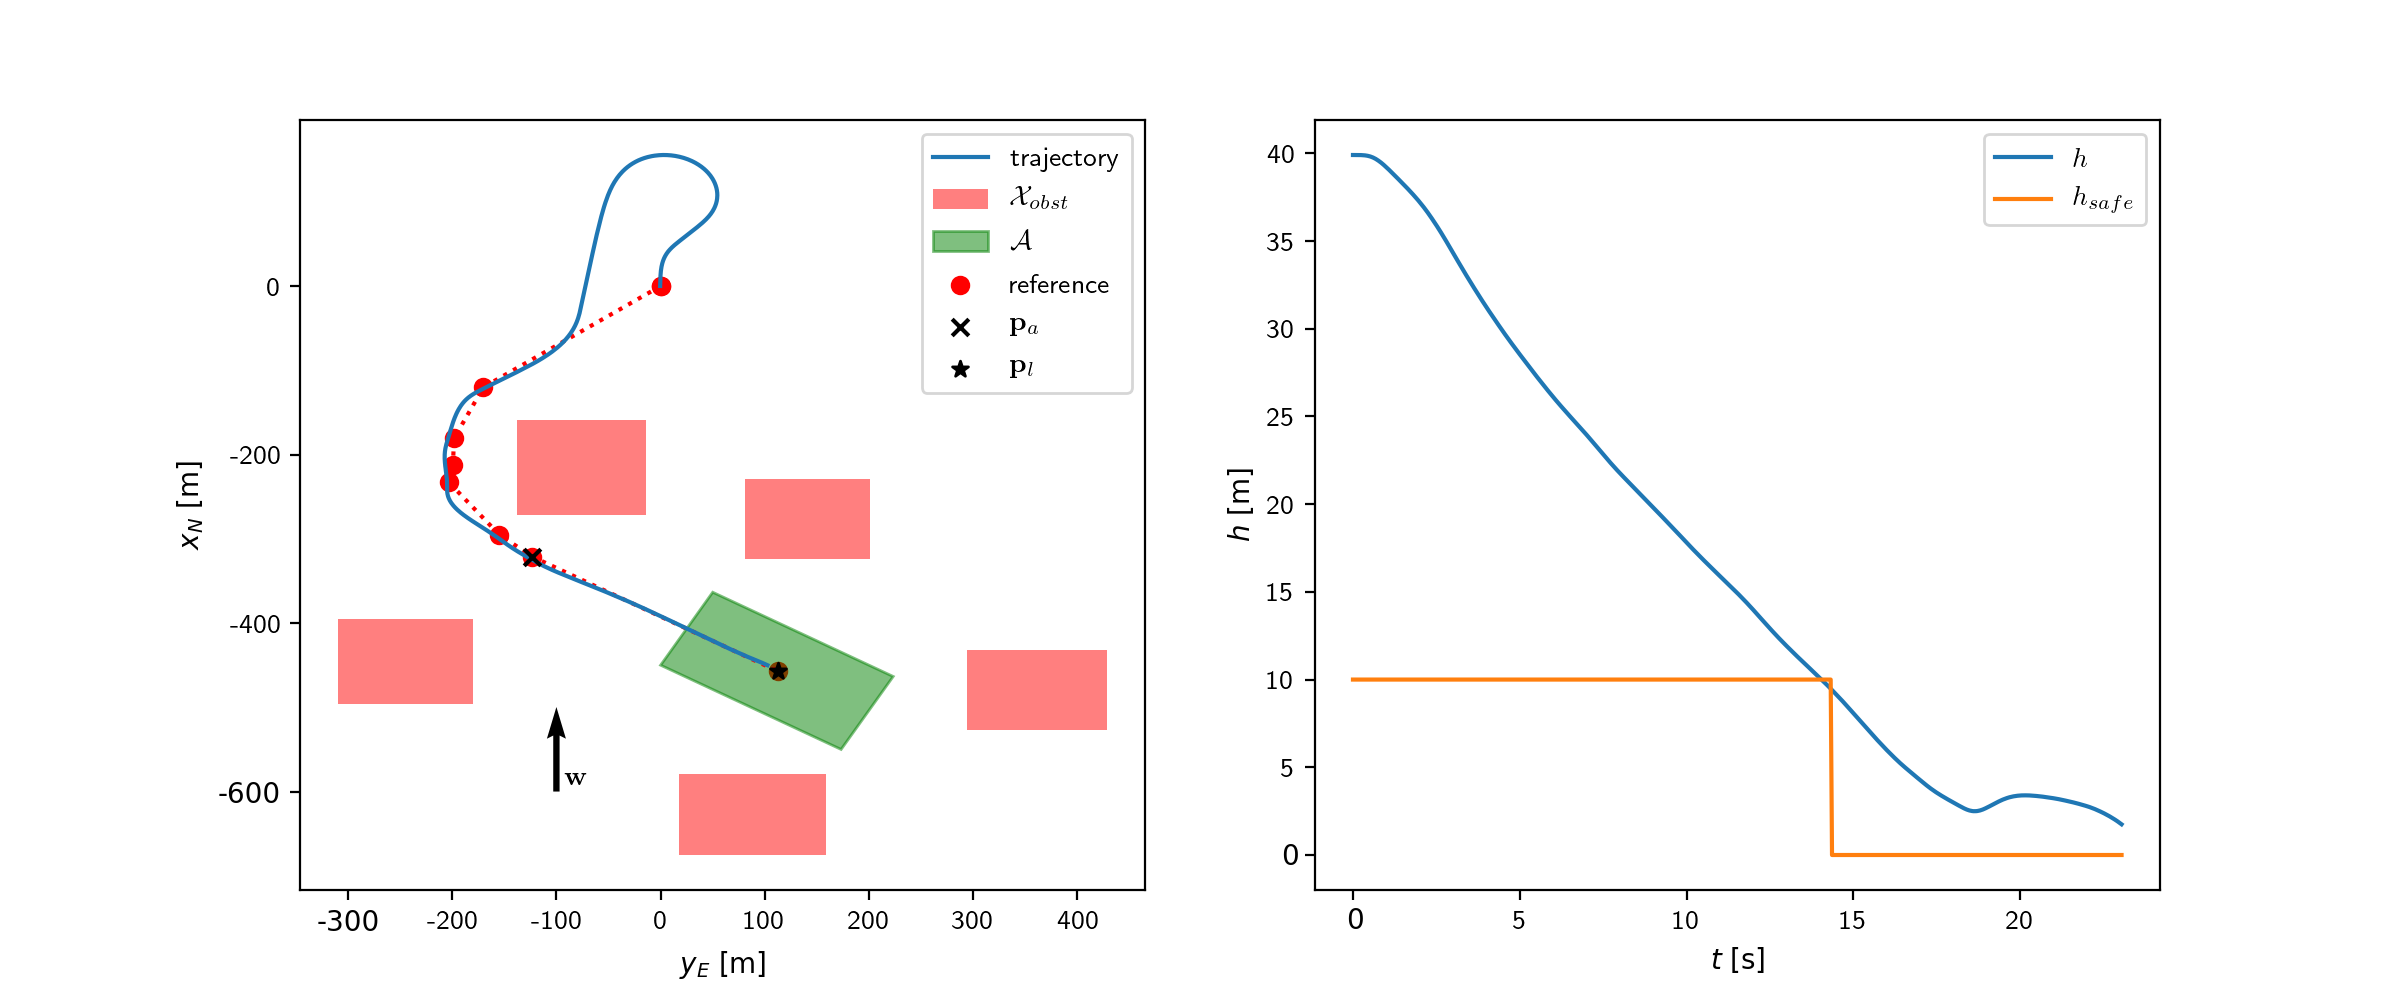
\includegraphics[width=1.3\textwidth]{sol_0}
    \caption{Landing sequence and altitude profile for $\winddir=0\degree$}
    \label{fig:sim_sol_0}
\end{figure}

\begin{figure}[H]
    \hspace{-0.15\textwidth}
    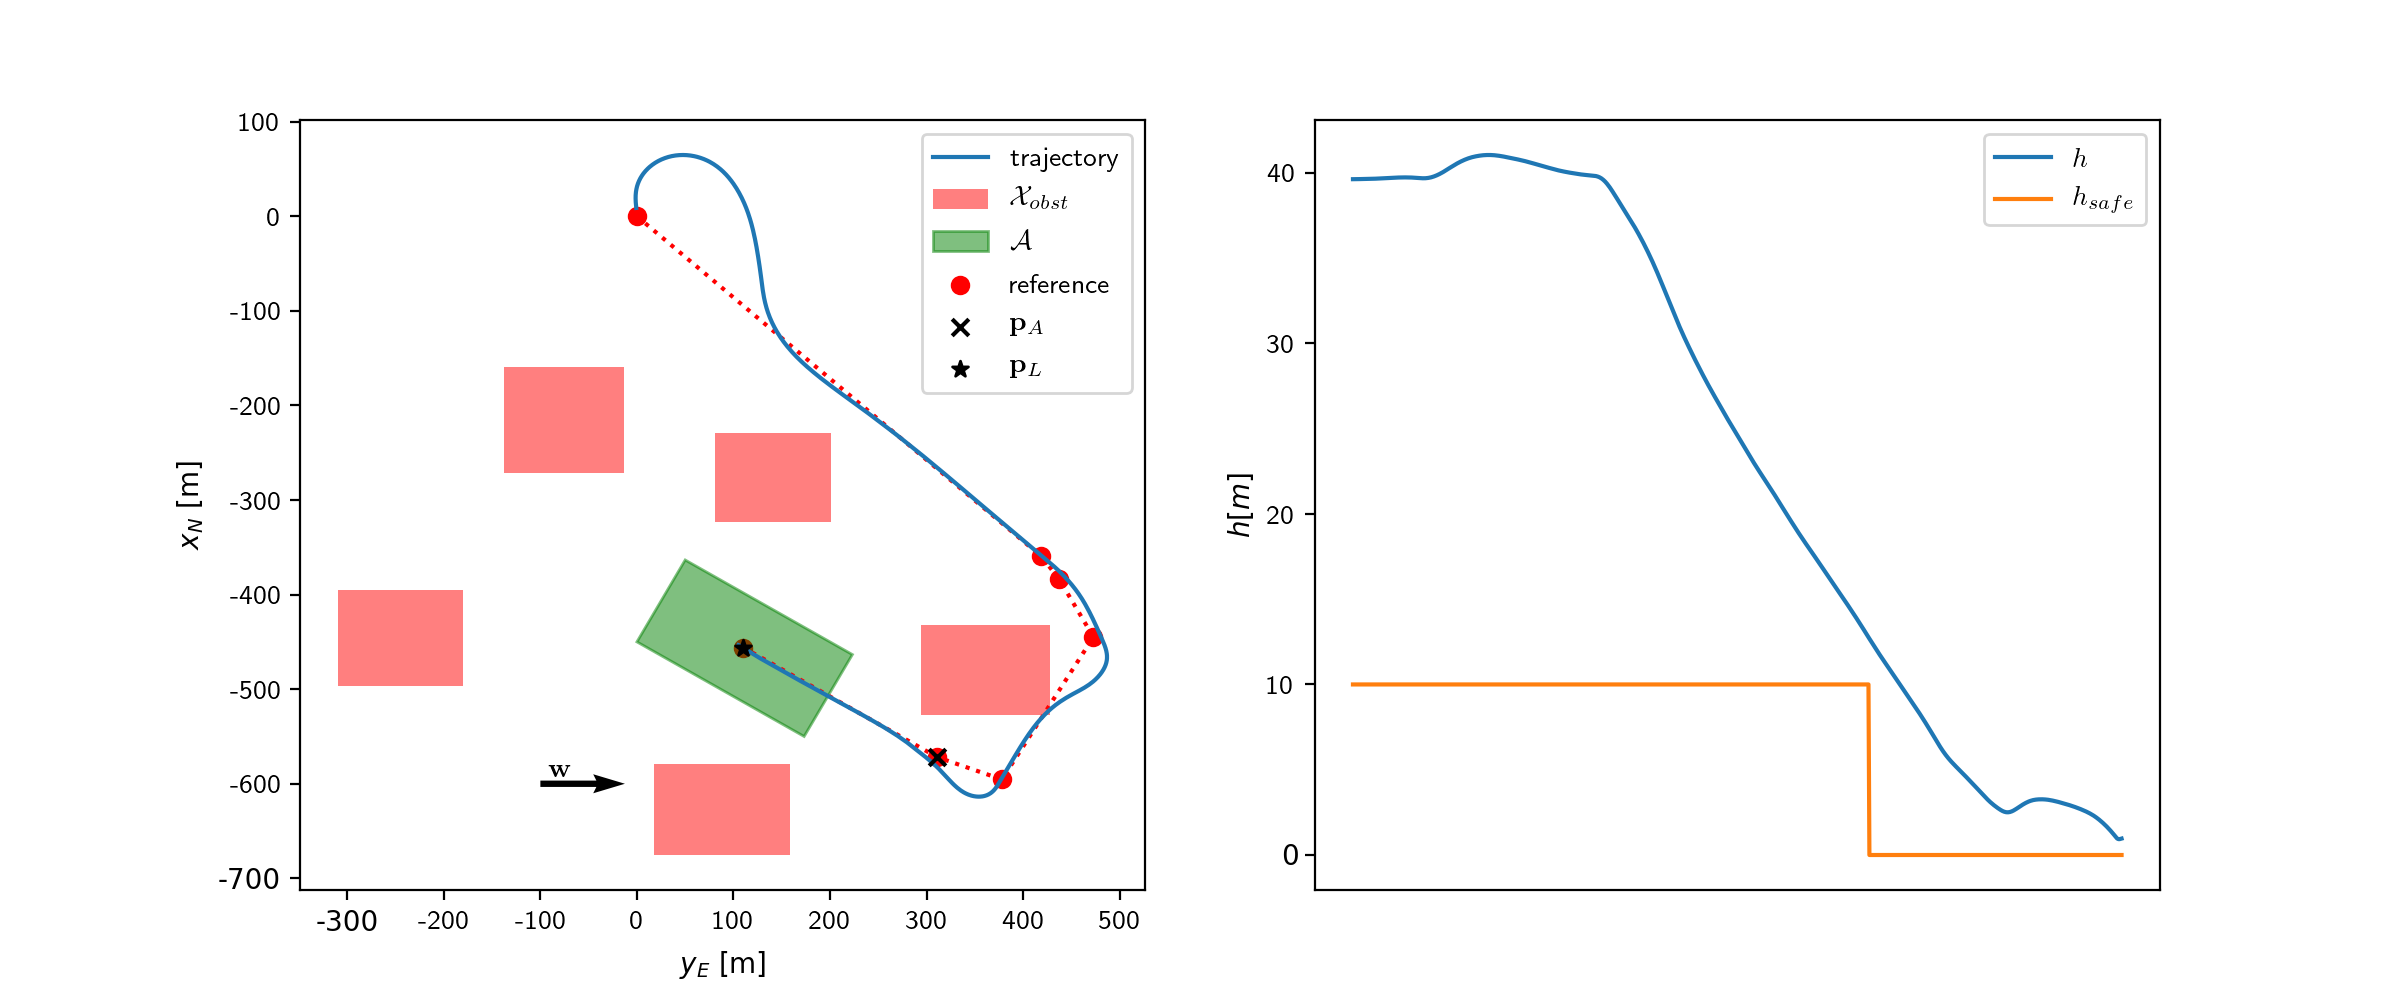
\includegraphics[width=1.3\textwidth]{sol_90}
    \caption{Landing sequence and altitude profile for $\winddir=90\degree$}
\end{figure}

\begin{figure}[H]
    \hspace{-0.15\textwidth}
    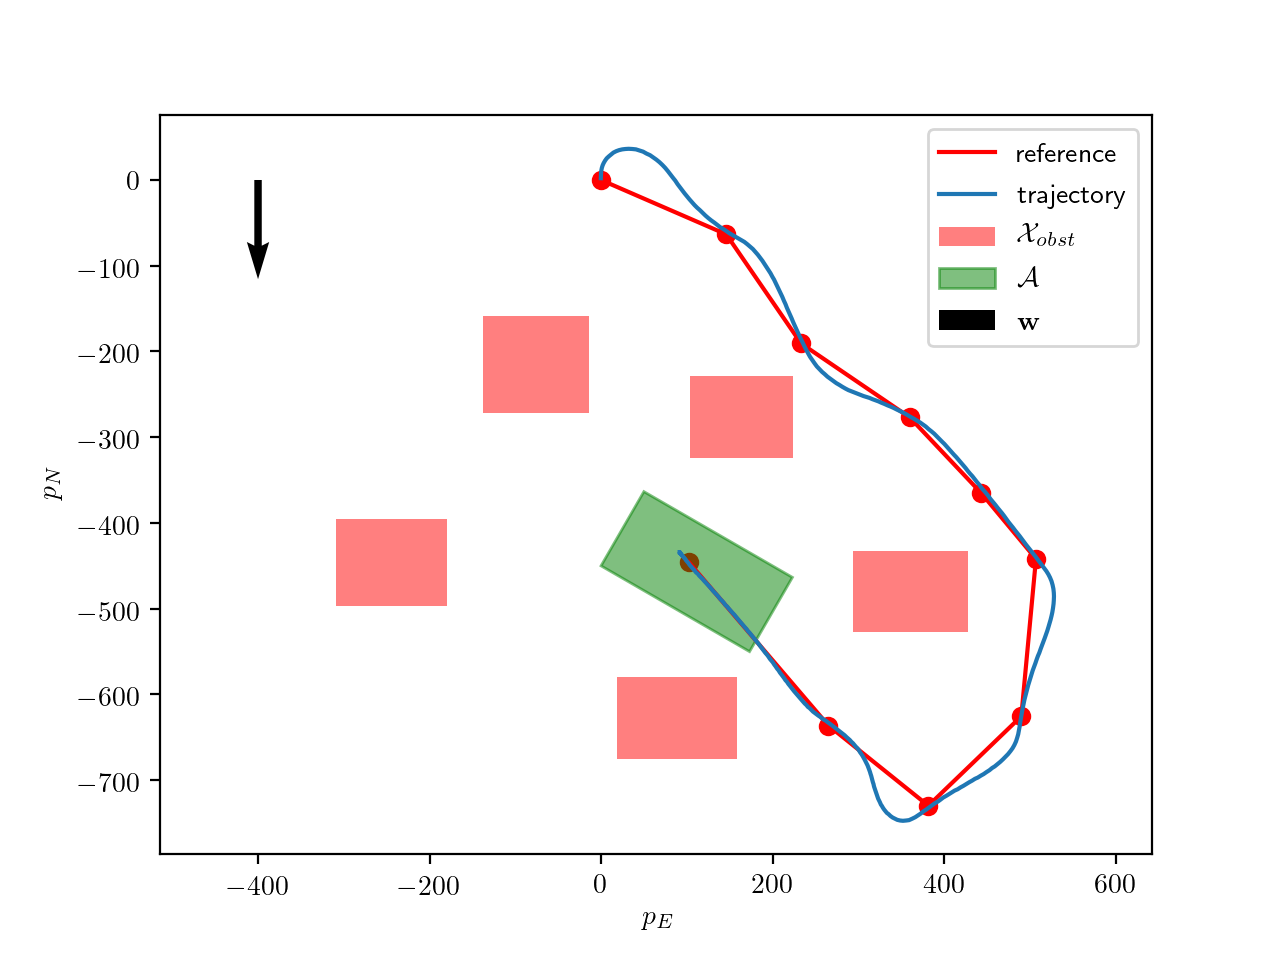
\includegraphics[width=1.3\textwidth]{sol_180}
    \caption{Landing sequence and altitude profile for $\winddir=180\degree$}
\end{figure}

\begin{figure}[H]
    \hspace{-0.15\textwidth}
    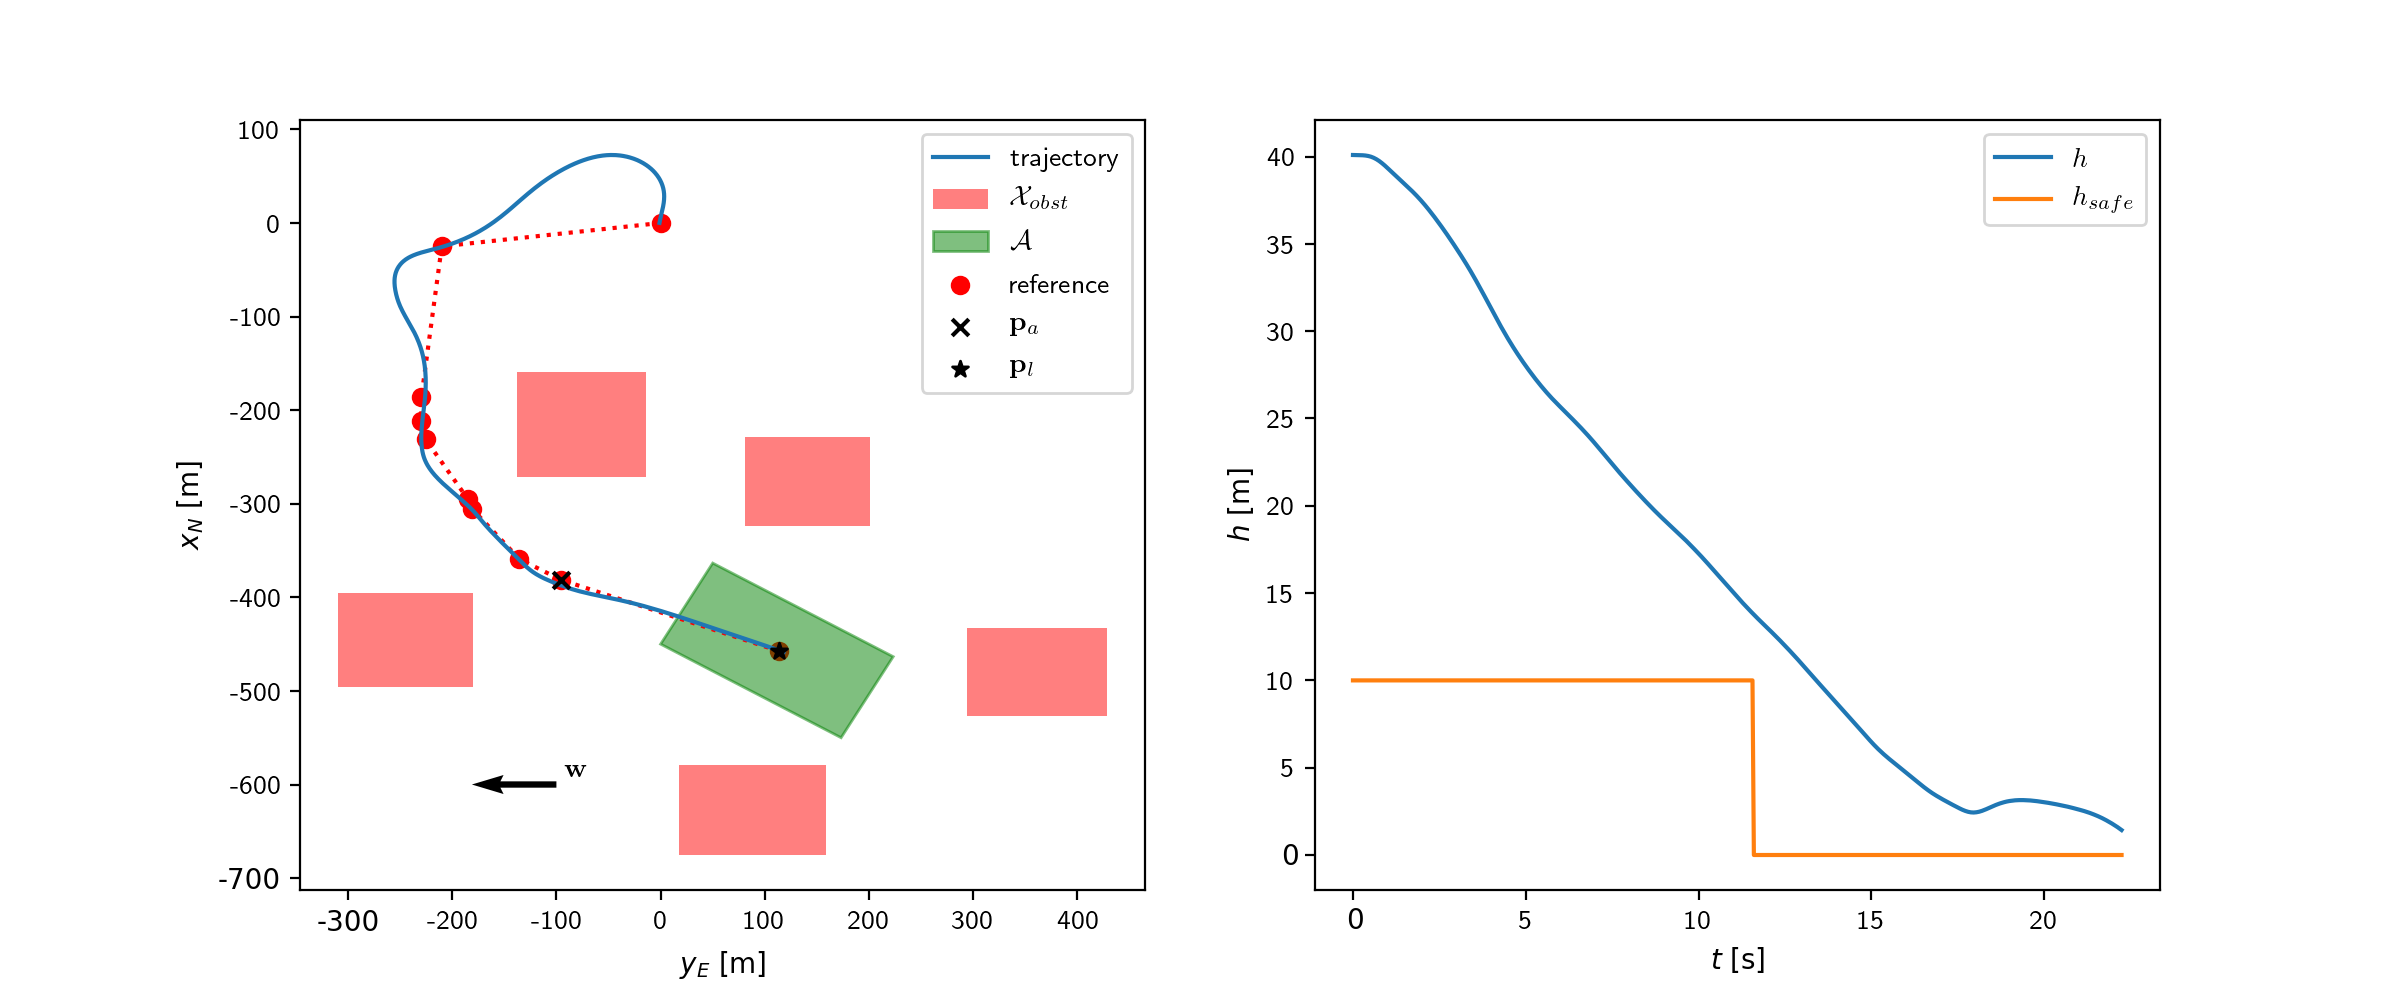
\includegraphics[width=1.3\textwidth]{sol_270}
    \caption{Landing sequence and altitude profile for $\winddir=270\degree$}
    \label{fig:sim_sol_270}
\end{figure}

\subsection{Discussion}
The results from simulation experiments indicate that the method successfully generates feasible landing 
sequences in different wind conditions. The distance between the planned and actual landing point is negligible relative to the total distance of the landing sequence.
The relative magnitude of the error in entry altitude is larger, but the \ac{uav} still manages to enter $\landing$ above the specified $h_{\text{safe}}$ in most cases. 
The error between calculated entry altitude and actual entry altitude seems quite constant, at least in the simulated evaluations summarized in Table \ref{tab:opt_land_param}. 
This implies that the error could be mitigated by estimating this offset and adding it to the desired $h_{\text{safe}}$. The error could also be mitigated by scaling the second term in the objective of 
Equation \eqref{eq:opt_problem_land} with some constant $\lambda_h>1$. The landing sequence generation is also quite fast, and a solution is found in well below 1 second in most cases.


\section{Real flight experiments}
In this section, setup and results of real flight experiments are presented.
\subsection{Experimental setup}
The \ac{uav} used during real flight experiments is shown in Figure \ref{fig:parrot}. This platform is based on a Parrot Disco airframe \cite{parrot}, 
which was modified to use the PixRacer autopilot \cite{pixracer} with Arduplane flight control software \cite{arduplane}. The \ac{uav} is also equipped with a 
Raspberry Pi 3B+ companion computer on which the landing system was deployed. The companion computer communicates with an external command and control interface using 
a 4G-LTE modem. The internal components of the \ac{uav} are shown in Figure \ref{fig:payload}, labeled as follows:
\begin{enumerate}
    \item Pitot tube sensor.
    \item 4G-LTE modem.
    \item Raspberry Pi companion computer.
    \item PixRacer autopilot.
    \item GPS receiver.
\end{enumerate}

\begin{figure}[H]
    \centering
    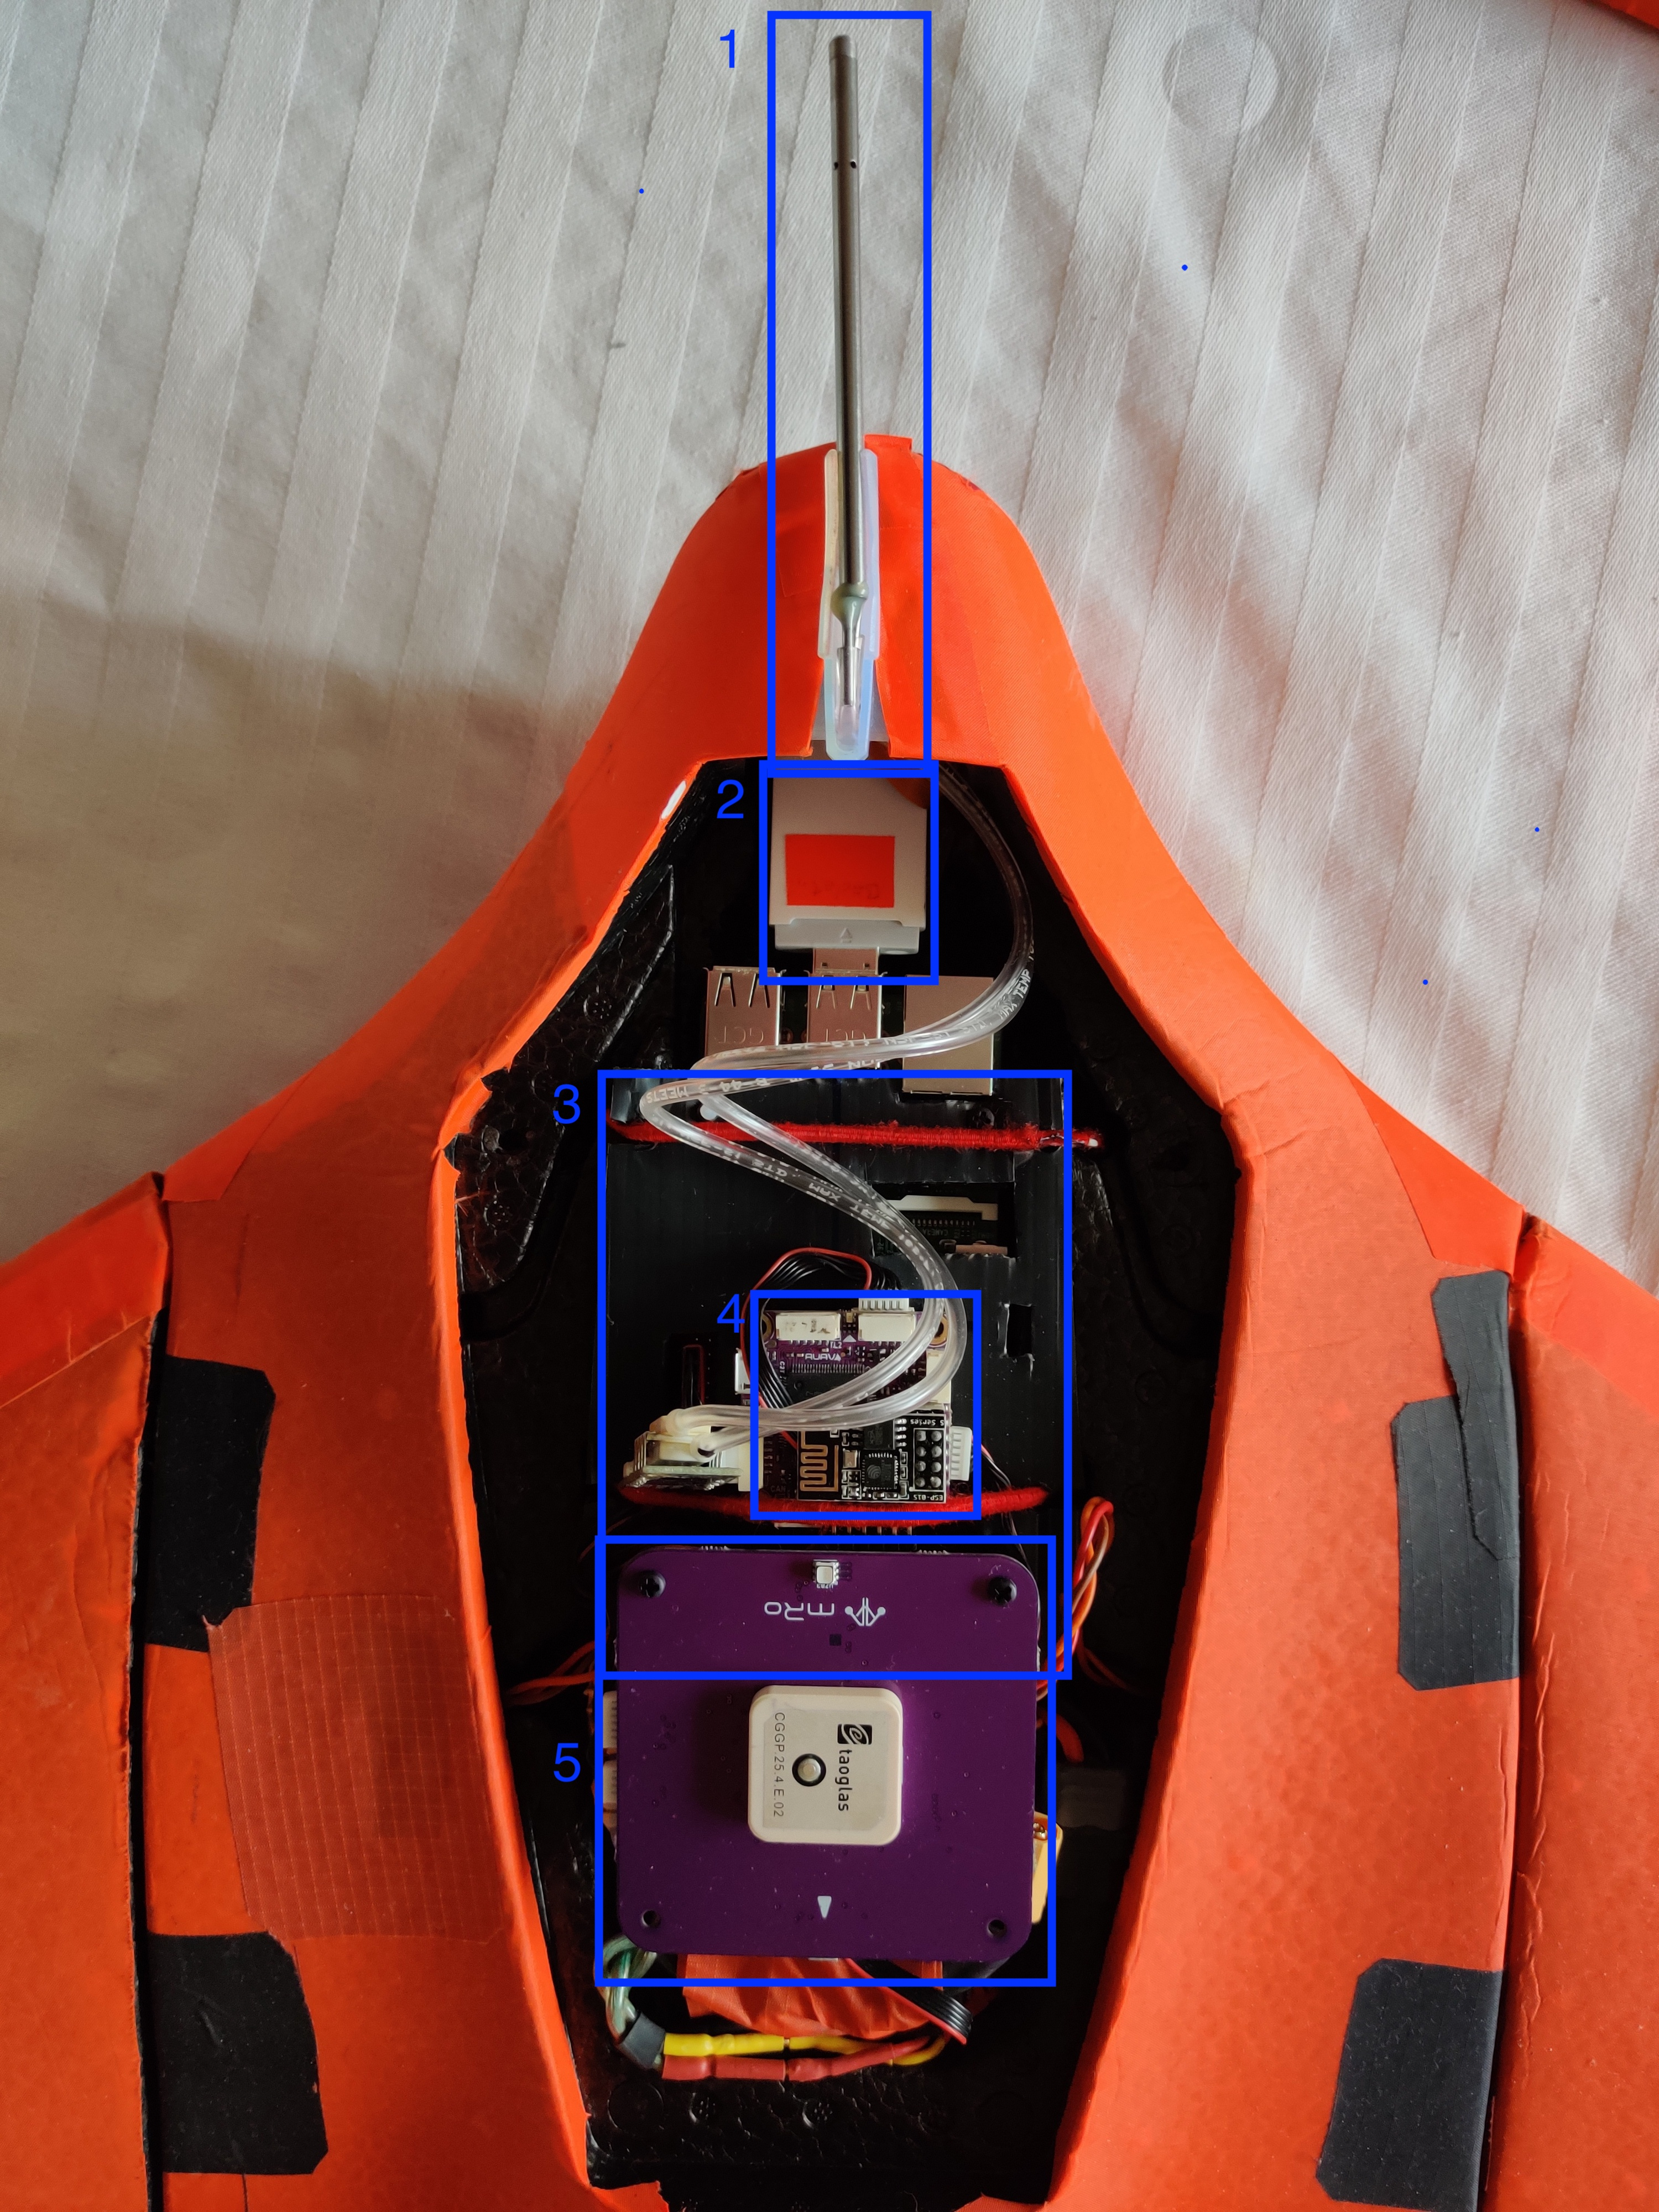
\includegraphics[width=.75\textwidth]{payload}
    \caption{Internal components of the \ac{uav} platform.}
    \label{fig:payload}
\end{figure}

\begin{figure}
    \begin{center}
        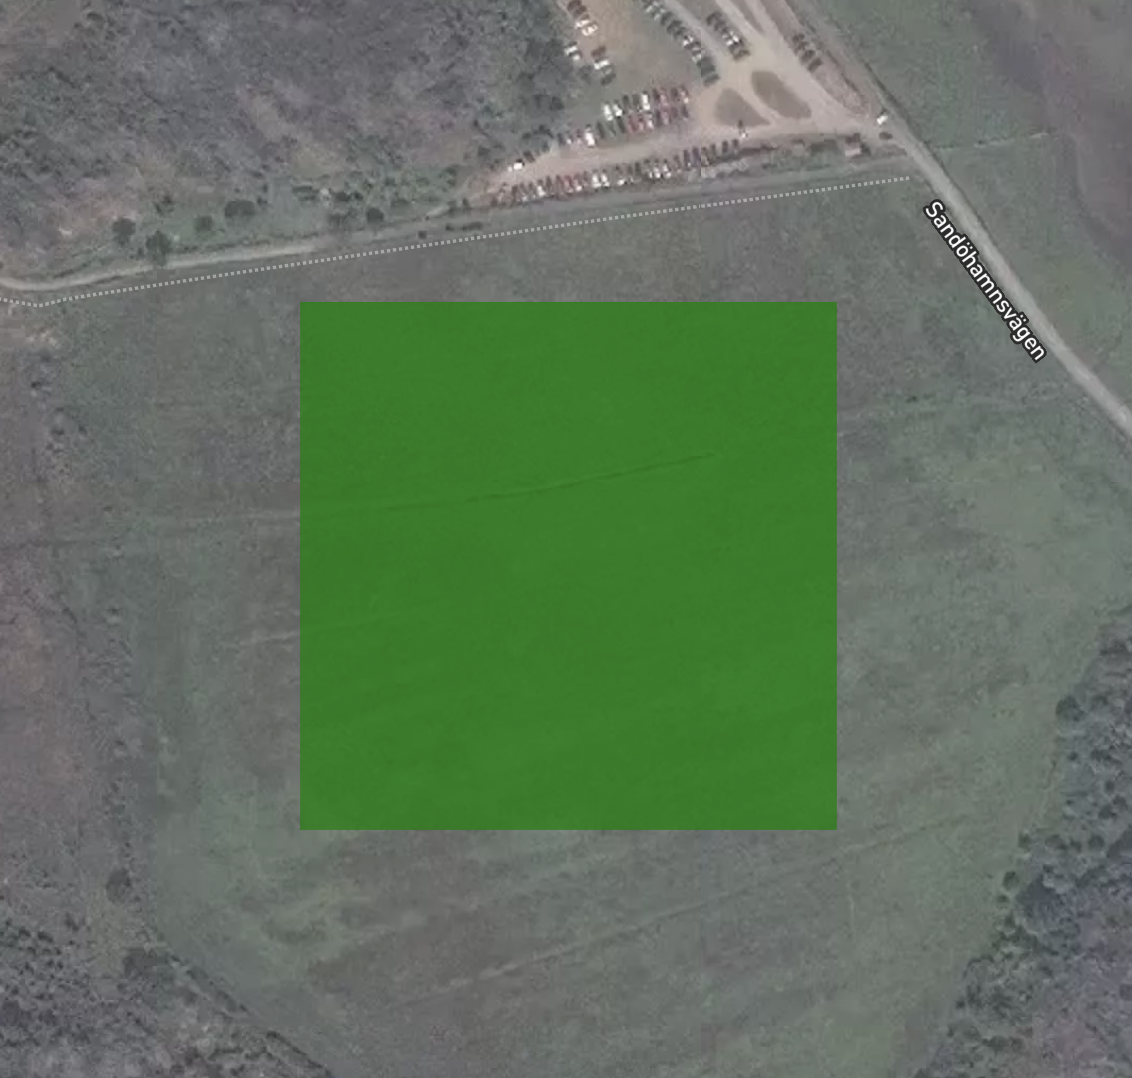
\includegraphics[width=.6\linewidth]{landing_map}
    \end{center}
    \caption{Landing area used for real flight experiments. Map data from Open Streetmap.}
    \label{fig:real_land_area}
\end{figure}

Experiments were conducted in an area near Longitude 11.929 and Latitude 54.486 south of Gothenburg, Sweden which is shown in Figure \ref{fig:real_land_area}.
The following procedure was followed during the experiments:
\begin{enumerate}
    \item Launch and takeoff with the \ac{uav}.
    \item Put the \ac{uav} in circular movement around a pre-defined coordinate $\vec{p}_{\text{loiter}}$, until the wind measurement has converged to an almost constant value.
    \item Compute $\vec{p}_a$ and $\vec{p}_l$ using the estimated wind direction and speed.
    \item Compute a waypoint mission from $x_0$ to $x_g=(x_{N,a},y_{E,a},\psi_l^*)$ with $x_0$ determined as described below.
    \item Send the computed mission to the autopilot and initiate mission execution.
\end{enumerate}

\subsection{Determining the starting state}
Since the motion planning algorithm assumes that the initial state of the \ac{uav} is exactly equal to the initial state used during planning, it is important 
that any positioning or heading errors are made as small as possible. This implies that $\vec{p}_{\text{loiter}}$ cannot be used directly as $x_0$ since the \ac{uav} circles around it, and thus 
the position and heading depends on when the landing sequence computation is initiated as well as the computation time which is uncertain.
Hence the starting state was determined by defining
\begin{equation}
    \vec{p}_{\pm90\degree} = \vec{p}_{\text{loiter}} + D\hat{r}_{\pm90\degree}
\end{equation}
where $\hat{r}_{\pm90\degree}$ is a unit vector pointing in the direction $\winddir\pm90\degree$ and $D$ was set to 100 m. The starting state was then set to
\begin{equation}
    x_0 = (x_{N,\pm90\degree},y_{E,\pm90\degree},\winddir\pm90\degree)
\end{equation}
depending on which of those points was closest to $\vec{p}_a$. This gives the \ac{uav} enough distance to reach the starting state exactly independent 
of where in the circular movement around $\vec{p}_{\text{loiter}}$ it is located when the mission is started.


\subsection{Results}
The trajectory and altitude profile of the \ac{uav} during a real landing is shown in Figure \ref{fig:real_land}. The estimated trajectory which was produced by the planner by forward simulation of the closed loop system is also shown. 
The reported wind speed and direction from the Swedish Meteorological and Hydrological Institute, SMHI at the time of the experiment was 
$\windspd=5$ m/s with gusts of 10 m/s, and $\winddir\approx120\degree$. The filtered estimates of both $\windspd$ and $\winddir$ during the flight are shown in Figure \ref{fig:real_wind}. The mean values used during planning were 
$\windspd=8.2$ m/s and $\winddir=118.8\degree$. The distance between planned and actual landing points in this experiment was $|R_l-R_l^*|=31$ m. 

 \begin{figure}
    \hspace{-0.15\textwidth}
    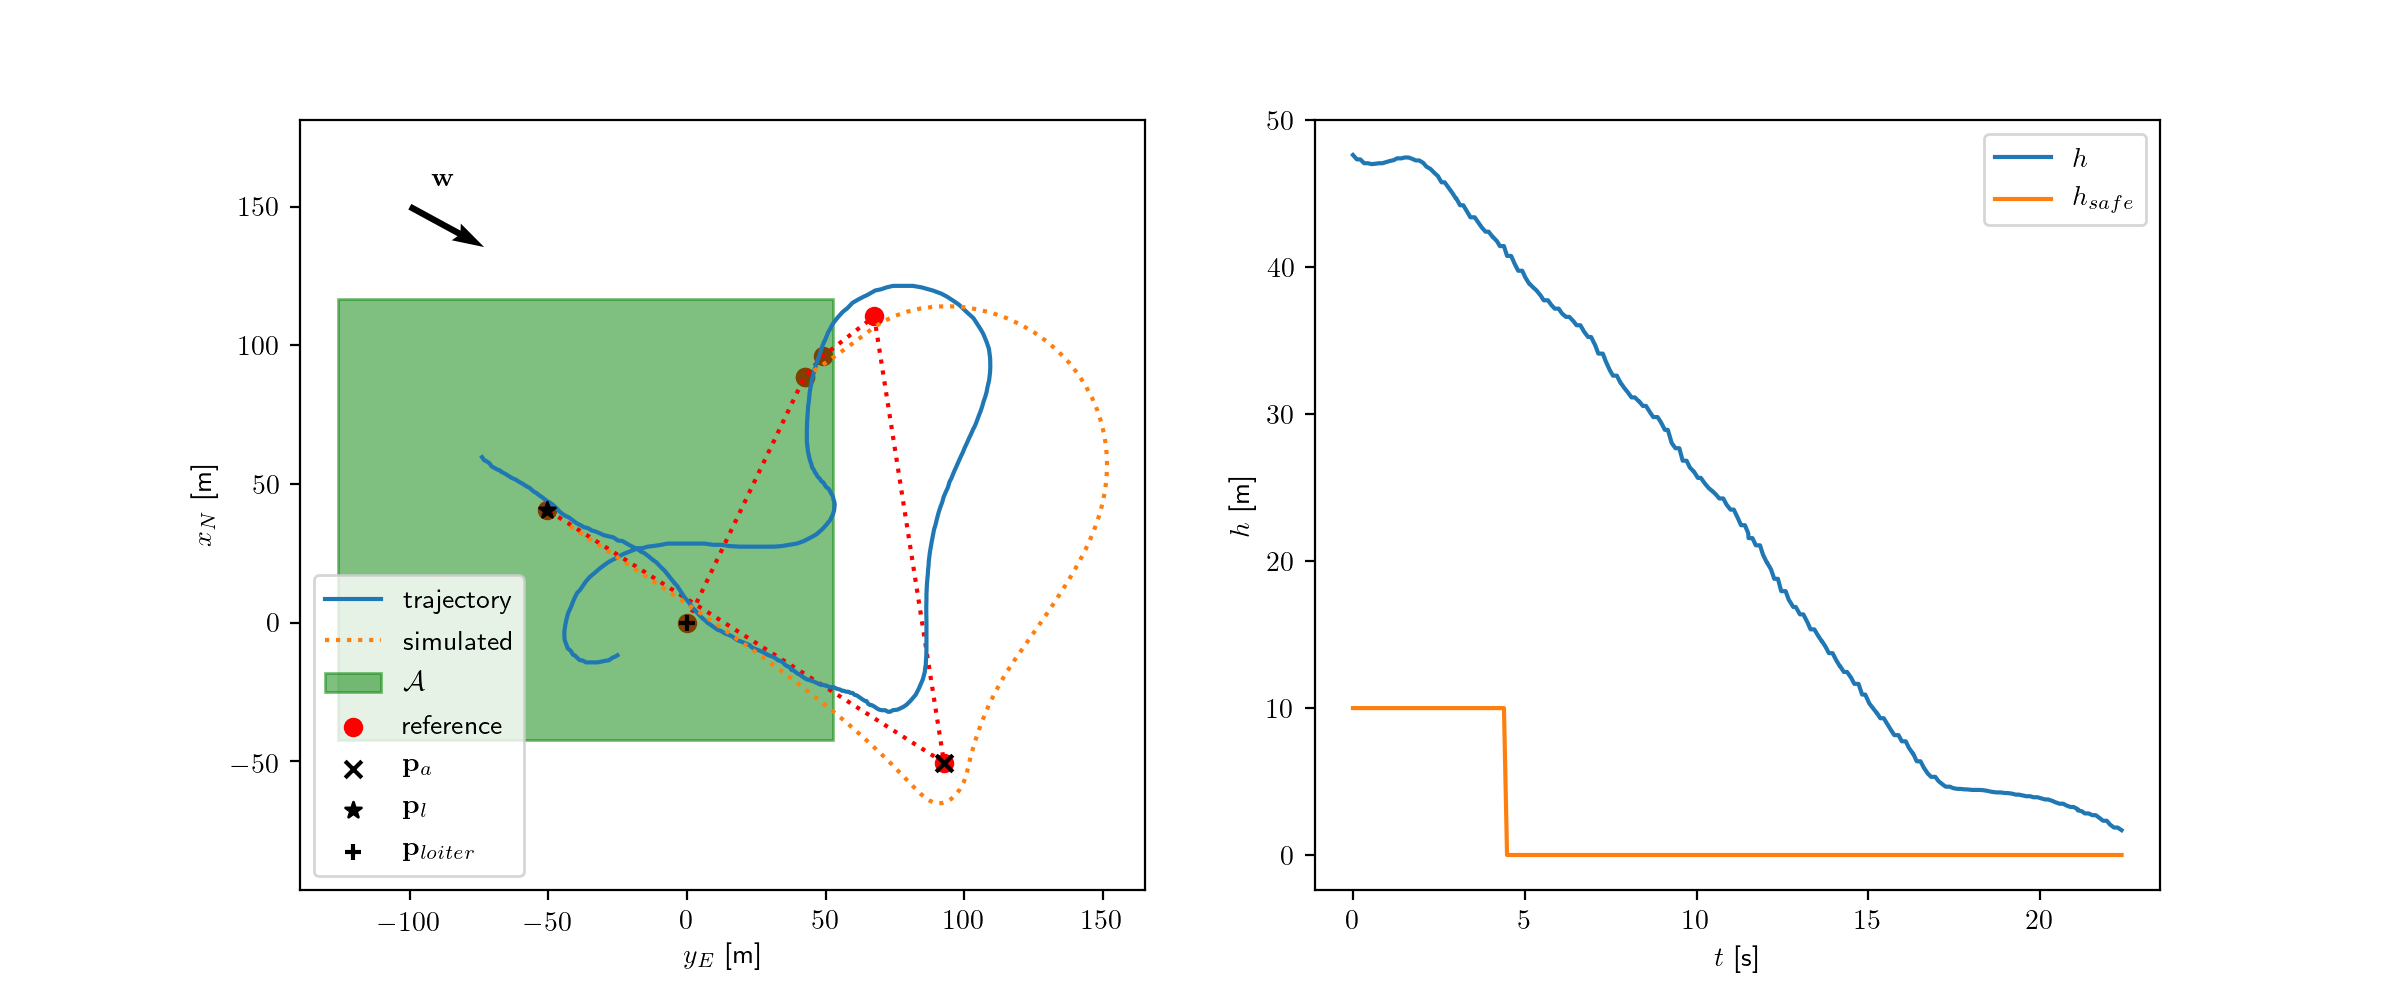
\includegraphics[width=1.3\textwidth]{real_flight}
     \caption{Trajectory and altitude profile of the real uav during execution of a landing sequence. The first waypoint is the point $\vec{p}_{\text{loiter}}$ which the \ac{uav} circles around while the landing sequence is calculated. 
     To compensate for the unpredictable initial heading when the landing sequence is initiated, the initial state is placed at a fixed distance from $\vec{p}_{\text{loiter}}$ in a direction perpendicular to the estimated $\winddir$.}
     \label{fig:real_land}
 \end{figure}

 \begin{figure}
    \hspace{-0.15\textwidth}
    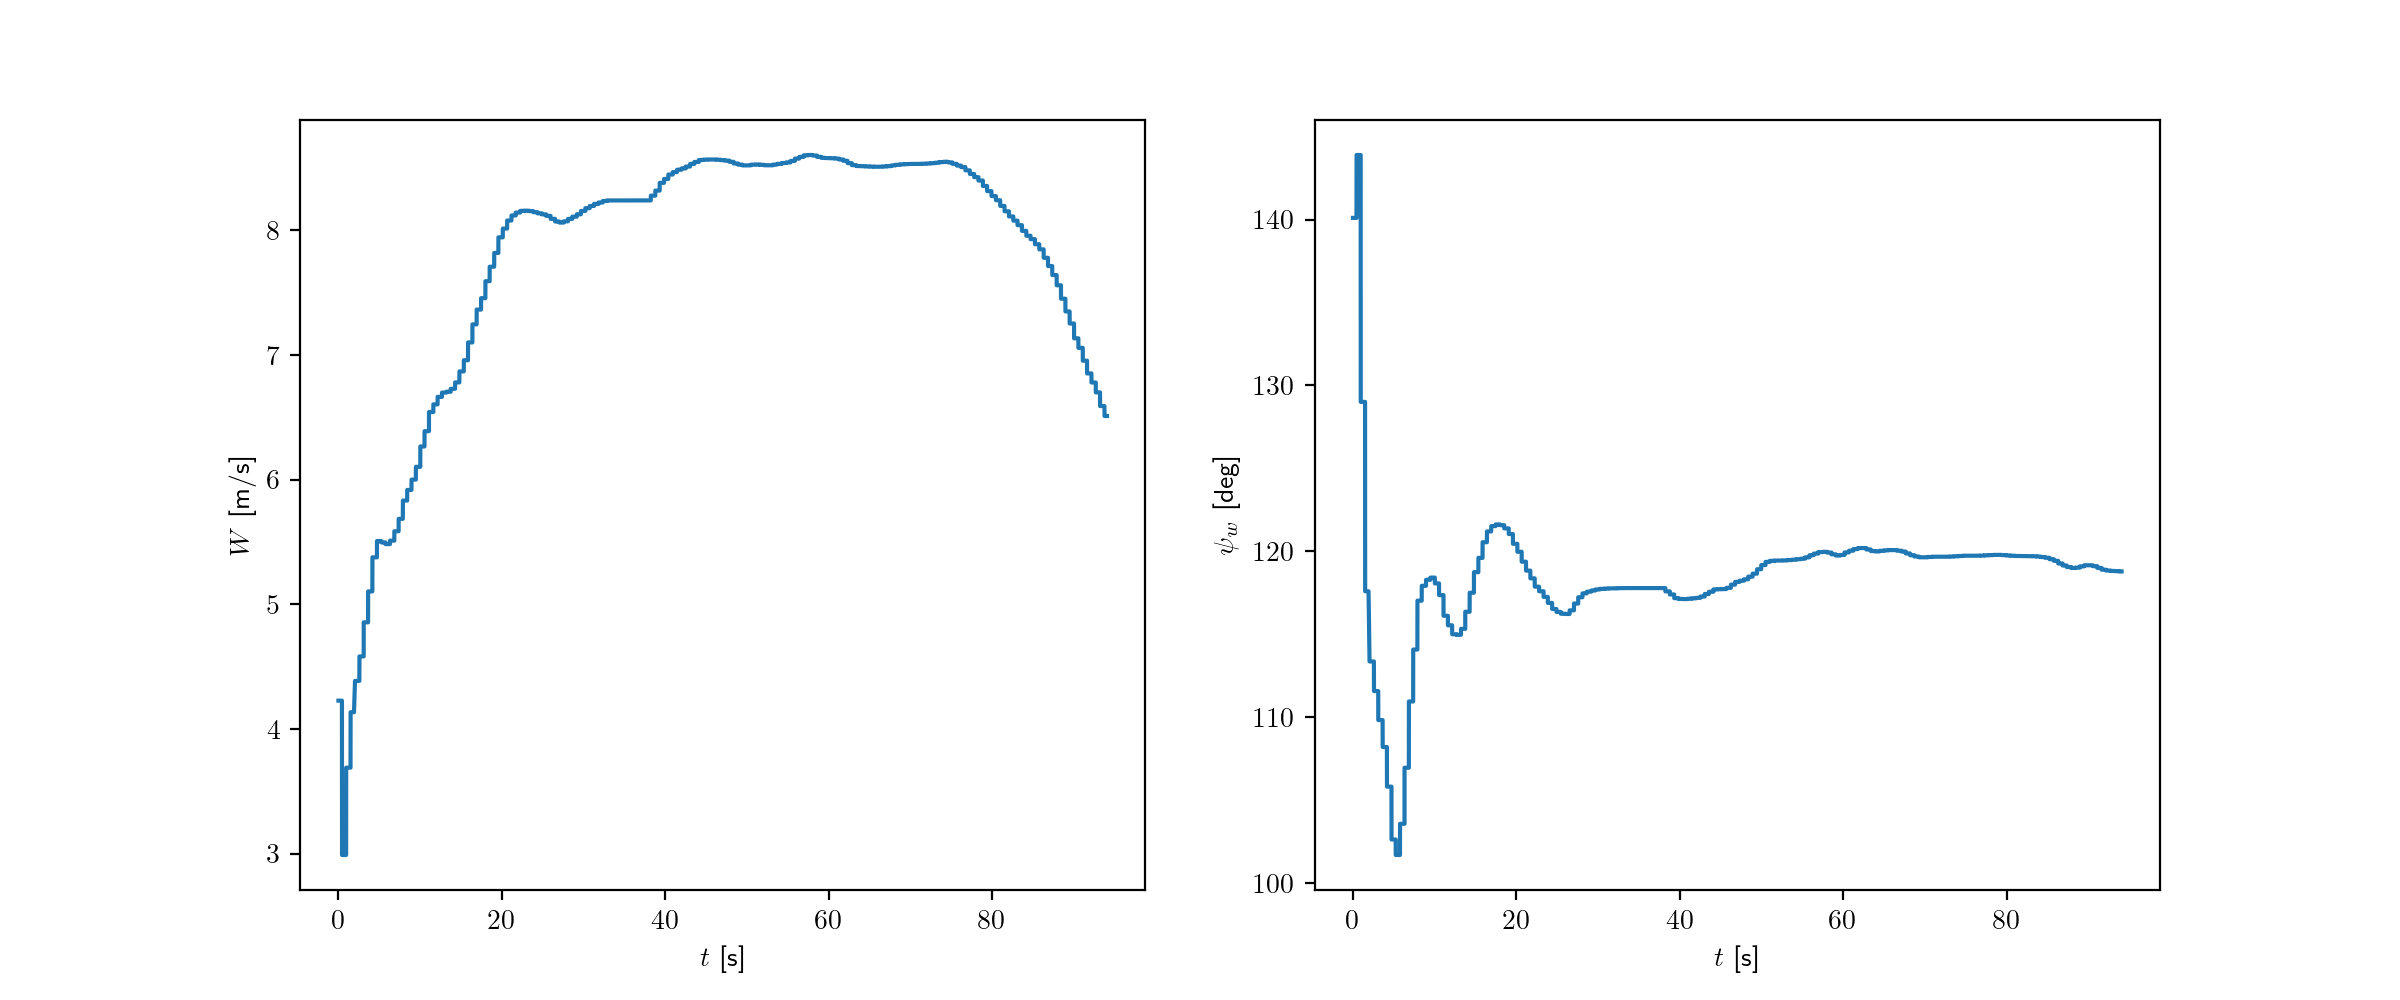
\includegraphics[width=1.3\textwidth]{real_wind}
    \caption{Filtered estimates of $\windspd$ and $\winddir$ during real flight experiment. Both plots show values from the entire duration of the flight, \ie\, from the moment the \ac{uav} takes of until it lands on the ground again.}
    \label{fig:real_wind}
 \end{figure}

 \subsection{Discussion}
In the real landing experiment, the distance between planned touchdown point and the actual was significantly larger than 
in the simulations. One reason for this, as can be seen in Figure \ref{fig:real_land}, is an inconsistency in value of the parameter $R_{\text{wp}}$, which determines how close the \ac{uav} should be to a target waypoint in 
order for it to be considered reached, between the planner and the autopilot. Since the expected wind speed was 5 m/s, the inputs used during planning were calculated for $\windspd\in[3.75, 6.25]$. The actual windspeed, however, turned out to be significantly higher. 
As such, using inputs computed for wind-speeds in an interval centered around $\bar{W}\approx8$ m/s would probably increase the accuracy further. It can also be noted that there is an overshoot in the trajectory following controller during the first 
straight-path segment. This might be caused by an unexpected wind gust, but such overshoots could probably be reduced by increasing the look-ahead distance $L_1$ of the controller.

To ensure a safe landing, the selected landing area for this experiment was quite large and thus the constraint on safe entry altitude was negligible. 
Nevertheless, the results are promising, and the method should be evaluated further by performing additional real flight experiments in more challenging scenarios.